\documentclass[10pt]{beamer}

% ============================================
% CODIFICACIÓN Y IDIOMA
% ============================================
\usepackage[utf8]{inputenc}
\usepackage[T1]{fontenc}
\usepackage[spanish]{babel}

% ============================================
% PAQUETES MATEMÁTICOS
% ============================================
\usepackage{amsmath,amsfonts,amssymb}
\usepackage{mathtools}

% ============================================
% GRÁFICOS Y COLORES
% ============================================
\usepackage{graphicx}
\usepackage{tikz}
\usepackage{pgfplots}
\pgfplotsset{compat=1.18}

% ============================================
% TABLAS
% ============================================
\usepackage{booktabs}
\usepackage{array}
\usepackage{multirow}
\usepackage{colortbl}

% ============================================
% COLORES PERSONALIZADOS (PALETA PASTEL)
% ============================================
\usepackage{xcolor}
\definecolor{celeste}{RGB}{135, 206, 235}
\definecolor{celesteBorde}{RGB}{100, 180, 220}
\definecolor{celesteClaro}{RGB}{230, 245, 255}
\definecolor{verdePastel}{RGB}{144, 238, 144}
\definecolor{naranjaPastel}{RGB}{255, 179, 71}
\definecolor{fucsiaPastel}{RGB}{255, 119, 188}
\definecolor{amarilloCaterpillar}{RGB}{255, 200, 50}
\definecolor{grisOscuro}{RGB}{60, 60, 60}
\definecolor{purpuraElectrico}{RGB}{138, 43, 226}
\definecolor{rojoDistintivo}{RGB}{220, 20, 60}

% ============================================
% TEMA BEAMER
% ============================================
\usetheme{Madrid}
\usecolortheme{default}
\setbeamertemplate{navigation symbols}{}

% Colores del tema adaptados a paleta pastel
\setbeamercolor{frametitle}{bg=celeste,fg=grisOscuro}
\setbeamercolor{title}{fg=grisOscuro}
\setbeamercolor{subtitle}{fg=grisOscuro}
\setbeamercolor{author}{fg=grisOscuro}
\setbeamercolor{date}{fg=grisOscuro}
\setbeamercolor{institute}{fg=grisOscuro}
\setbeamercolor{block title}{bg=celeste,fg=grisOscuro}
\setbeamercolor{block body}{bg=celesteClaro,fg=grisOscuro}
\setbeamercolor{block title example}{bg=verdePastel,fg=grisOscuro}
\setbeamercolor{block body example}{bg=verdePastel!20,fg=grisOscuro}
\setbeamercolor{block title alerted}{bg=naranjaPastel,fg=grisOscuro}
\setbeamercolor{block body alerted}{bg=naranjaPastel!20,fg=grisOscuro}
\setbeamercolor{item}{fg=celesteBorde}
\setbeamercolor{footline}{bg=celeste,fg=grisOscuro}

% ============================================
% PIE DE PÁGINA PERSONALIZADO
% ============================================
\setbeamertemplate{footline}{
  \leavevmode%
  \hbox{%
  \begin{beamercolorbox}[wd=.333333\paperwidth,ht=2.25ex,dp=1ex,center]{author in head/foot}%
    \usebeamerfont{author in head/foot}\insertshortauthor
  \end{beamercolorbox}%
  \begin{beamercolorbox}[wd=.333333\paperwidth,ht=2.25ex,dp=1ex,center]{title in head/foot}%
    \usebeamerfont{title in head/foot}\insertshorttitle
  \end{beamercolorbox}%
  \begin{beamercolorbox}[wd=.333333\paperwidth,ht=2.25ex,dp=1ex,right]{date in head/foot}%
    \usebeamerfont{date in head/foot}
    \colorbox{amarilloCaterpillar}{\textcolor{grisOscuro}{\insertframenumber{} / \inserttotalframenumber}}\hspace*{2ex}
  \end{beamercolorbox}}%
  \vskip0pt%
}

% ============================================
% INFORMACIÓN DEL DOCUMENTO
% ============================================
\title[Unidad 4: Normal y Exponencial]{Unidad 4}
\subtitle{Distribución de Probabilidades para Variable Aleatoria Continua}
\author[MSc. Anselmo Salguero Arano]{MSc. Anselmo Salguero Arano}
\institute[UAGRM - Contaduría Pública]{%
  Universidad Autónoma Gabriel René Moreno\\
  Facultad de Ciencias Contables, Auditoría, Sistemas de Control de Gestión y Finanzas\\
  Carrera de Contaduría Pública\\
  Estadística II -- MAT-260
}
\date{2025}

% ============================================
% INICIO DEL DOCUMENTO
% ============================================
\begin{document}

% ============================================
% PORTADA
% ============================================
\begin{frame}[plain]
\begin{center}
\vspace{0.5cm}

\includegraphics[width=0.30\linewidth]{Logouagrm.png}
\hspace{0.5cm}

\includegraphics[width=0.30\linewidth]{Logocont.png}

\vspace{0.8cm}
{\Huge\textcolor{celeste}{\textbf{Estadística II}}}

\vspace{0.3cm}
{\LARGE\textcolor{grisOscuro}{Unidad 4}}

\vspace{0.2cm}
{\Large\textcolor{grisOscuro}{Distribución de Probabilidades\\para Variable Aleatoria Continua}}

\vspace{0.8cm}
{\large\textcolor{grisOscuro}{MSc. Anselmo Salguero Arano}}

\vspace{0.2cm}
{\normalsize\textcolor{grisOscuro}{Docente -- Estadística II}}

\vspace{0.5cm}
{\footnotesize\textcolor{grisOscuro}{Universidad Autónoma Gabriel René Moreno\\
Facultad de Ciencias Contables, Auditoría, Sistemas de Control de Gestión y Finanzas\\
Carrera de Contaduría Pública}}

\vspace{0.3cm}
{\footnotesize\textcolor{celesteBorde}{Santa Cruz -- Bolivia}}
\end{center}
\end{frame}

% ============================================
% CONTENIDO DE LA UNIDAD
% ============================================
\begin{frame}{Contenido de la Unidad 4}
\begin{block}{Temas a desarrollar}
\begin{enumerate}
  \item \textbf{Variable Aleatoria Continua:} Definición y propiedades
  \item \textbf{Función de Densidad de Probabilidad:} $f(x)$
  \item \textbf{Distribución Normal:} Campana de Gauss
  \item \textbf{Estandarización:} $Z = \dfrac{X - \mu}{\sigma}$
  \item \textbf{Uso de Tablas Z:} Lind, p. 782
  \item \textbf{Distribución Exponencial:} Tiempos de espera
  \item \textbf{Ejercicios Resueltos:} Paso a paso
\end{enumerate}
\end{block}

\begin{exampleblock}{Referencias}
\begin{itemize}
  \item Texto: MSc. Anselmo Salguero Arano -- Unidad 4
  \item Lind, Marchal, Wathen. \textit{Estadística Aplicada a los Negocios y la Economía}. 15 Ed. McGraw-Hill.
  \item Capítulo 7: Distribuciones de Probabilidad Continua (pp. 222--264)
  \item Apéndice B: Tablas (p. 782)
\end{itemize}
\end{exampleblock}
\end{frame}

% ============================================
% VARIABLE ALEATORIA CONTINUA
% ============================================
\begin{frame}{Variable Aleatoria Continua}
\begin{block}{Definición}
Una \textbf{variable aleatoria continua} puede tomar \textbf{cualquier valor} dentro de un intervalo específico. A diferencia de las variables discretas, no existen ``vacíos'' entre los valores posibles.
\end{block}

\vspace{0.2cm}
\begin{exampleblock}{Ejemplos de Variables Continuas}
\begin{itemize}
  \item Peso de un estudiante
  \item Monto del impuesto sobre la renta
  \item Precipitación anual
  \item Tiempo de espera en una fila
  \item Temperatura ambiente
\end{itemize}
\end{exampleblock}

\vspace{0.2cm}
\begin{alertblock}{Nota importante}
Para variables continuas, la probabilidad de que $X$ tome un \textbf{valor exacto} es \textbf{cero}:
$$P(X = x) = 0$$
La probabilidad se calcula para \textbf{intervalos}: $P(a \leq X \leq b)$
\end{alertblock}
\end{frame}

% ============================================
% DISTRIBUCIONES CONTINUAS
% ============================================
\begin{frame}{Distribuciones Continuas de Probabilidad}
\begin{block}{Principales distribuciones continuas}
\begin{enumerate}
  \item \textbf{Normal o Estándar} -- Campana de Gauss
  \item \textbf{Exponencial} -- Tiempos de espera y vida útil
\end{enumerate}
\end{block}

\vspace{0.3cm}
\begin{center}
\begin{tikzpicture}[
  nivel1/.style={rectangle, draw=celesteBorde, fill=celesteClaro, rounded corners, 
    minimum width=3cm, minimum height=0.8cm, align=center, font=\small},
  nivel2/.style={rectangle, draw=celesteBorde, fill=celeste!30, rounded corners,
    minimum width=2.2cm, minimum height=0.6cm, align=center, font=\footnotesize},
  arrow/.style={->, thick, celesteBorde}
]
\node[nivel1] (va) at (0,0) {Variable Aleatoria};
\node[nivel2] (disc) at (-2.5,-1.2) {Discreta};
\node[nivel2] (cont) at (2.5,-1.2) {Continua};

\node[nivel2, fill=verdePastel!40] (norm) at (0,-2.5) {Normal};
\node[nivel2, fill=fucsiaPastel!40] (exp) at (2.5,-2.5) {Exponencial};

\draw[arrow] (va) -- (disc);
\draw[arrow] (va) -- (cont);
\draw[arrow] (cont) -- (norm);
\draw[arrow] (cont) -- (exp);
\end{tikzpicture}
\end{center}

\vspace{0.3cm}
\begin{alertblock}{Importante}
Existen \textbf{tablas de probabilidad} para la distribución normal estándar, haciendo que resulte \textbf{innecesario} el método de la integración para determinar las áreas bajo la curva.
\end{alertblock}
\end{frame}

% ============================================
% FUNCIÓN DE DENSIDAD
% ============================================
\begin{frame}{Función de Densidad de Probabilidad}
\begin{block}{Definición}
La \textbf{función de densidad de probabilidad} $f(x)$ describe la forma de la distribución continua. El área bajo la curva entre dos valores $a$ y $b$ da la probabilidad:
\end{block}

\begin{center}
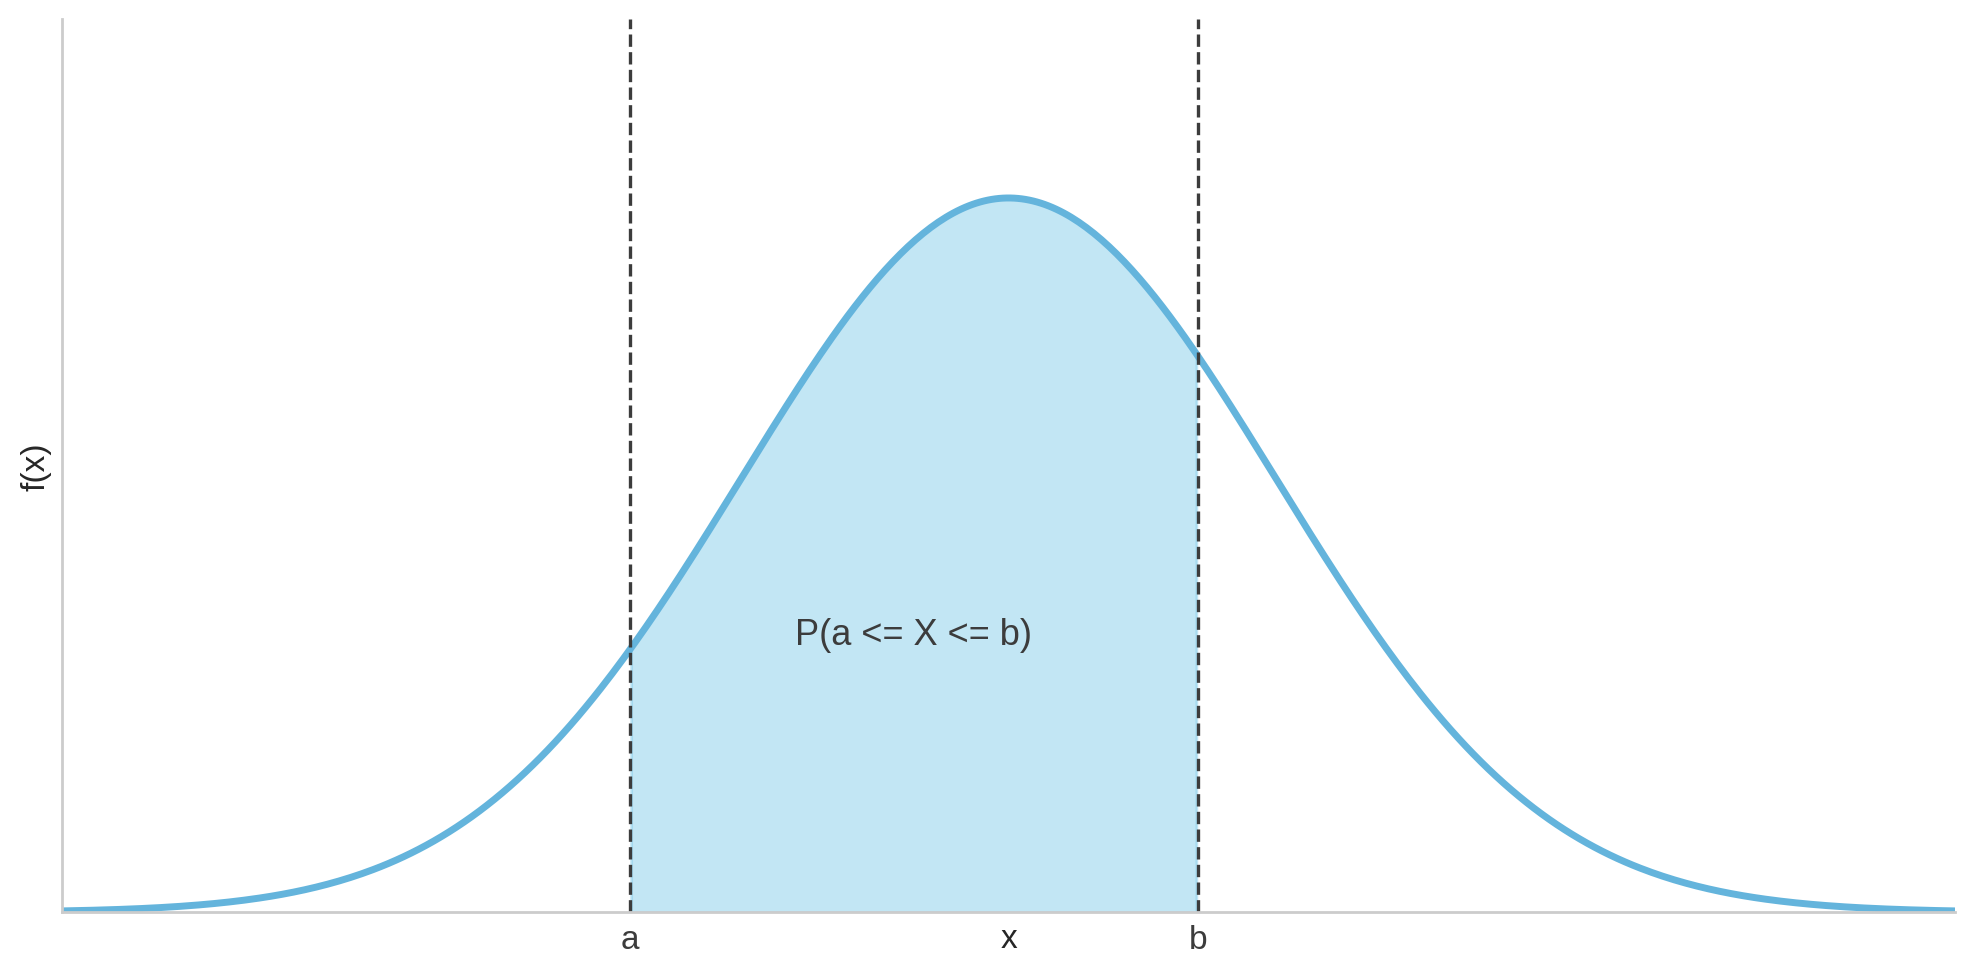
\includegraphics[width=0.75\linewidth]{fig_densidad_area.png}
\end{center}

\begin{alertblock}{Propiedad fundamental}
$$P(a \leq X \leq b) = \int_a^b f(x)\,dx = \text{Área bajo la curva entre } a \text{ y } b$$
El \textbf{área total} bajo la curva siempre es igual a \textbf{1}:
$$\int_{-\infty}^{+\infty} f(x)\,dx = 1$$
\end{alertblock}
\end{frame}

% ============================================
% DISTRIBUCIÓN NORMAL - DEFINICIÓN
% ============================================
\begin{frame}{Distribución Normal o Estándar}
\begin{block}{Definición (Texto Anselmo Salguero)}
La gráfica de una distribución normal es una \textbf{curva en forma de campana} que se extiende \textbf{indefinidamente} en ambos sentidos.
\end{block}

\vspace{0.2cm}
\begin{exampleblock}{Notación}
Si $X$ sigue una distribución normal con media $\mu$ y desviación estándar $\sigma$:
$$X \sim N(\mu, \sigma)$$
\end{exampleblock}

\vspace{0.2cm}
\begin{block}{Características}
\begin{itemize}
  \item Simétrica respecto a la media $\mu$
  \item Asintótica al eje $x$ (nunca lo toca)
  \item Puntos de inflexión en $\mu \pm \sigma$
  \item Área total = 1
\end{itemize}
\end{block}
\end{frame}

% ============================================
% IMPORTANCIA DE LA NORMAL - PARTE 1
% ============================================
\begin{frame}{Importancia de la Distribución Normal (I)}
\begin{block}{¿Por qué es tan importante?}
\begin{enumerate}
  \item \textbf{Procesos naturales:} Muchas mediciones en procesos aleatorios siguen esta distribución.
  \item \textbf{Aproximación:} Las probabilidades normales pueden aproximar otras distribuciones:
  \begin{itemize}
    \item Distribución Binomial
    \item Distribución de Poisson
  \end{itemize}
\end{enumerate}
\end{block}

\vspace{0.2cm}
\begin{exampleblock}{Aplicaciones en Contaduría}
\begin{itemize}
  \item Análisis de rendimientos de inversiones
  \item Control de calidad en procesos de producción
  \item Predicción de flujos de caja
  \item Evaluación de riesgos financieros
\end{itemize}
\end{exampleblock}
\end{frame}

% ============================================
% IMPORTANCIA DE LA NORMAL - PARTE 2
% ============================================
\begin{frame}{Importancia de la Distribución Normal (II)}
\begin{block}{Teorema Central del Límite}
Las distribuciones de la media muestral y la proporción muestral tienen distribución normal cuando el tamaño de la muestra es grande ($n \geq 30$), \textbf{sin importar} la forma de la distribución de la población de origen.
\end{block}

\vspace{0.3cm}
\begin{center}
\begin{tikzpicture}
\draw[celesteBorde, thick, rounded corners, fill=celesteClaro] (0,0) rectangle (10,1.5);
\node at (5,0.9) {\large Si $n \geq 30$, entonces $\bar{X} \sim N\left(\mu, \dfrac{\sigma}{\sqrt{n}}\right)$};
\node at (5,0.4) {\normalsize Independientemente de la distribución original de la población};
\end{tikzpicture}
\end{center}
\end{frame}

% ============================================
% FÓRMULA DE LA NORMAL
% ============================================
\begin{frame}{Función de Densidad Normal}
\begin{block}{Fórmula de la Distribución Normal}
\begin{center}
\Large
$$f(x) = \frac{1}{\sigma\sqrt{2\pi}} \cdot e^{-\frac{1}{2}\left(\frac{x-\mu}{\sigma}\right)^2}$$
\end{center}
\end{block}

\vspace{0.2cm}
\begin{exampleblock}{Donde:}
\begin{center}
\begin{tabular}{ll}
\toprule
\textbf{Símbolo} & \textbf{Significado} \\
\midrule
$e$ & $2{,}7183$ (base de logaritmos naturales) \\
$\pi$ & $3{,}1416$ \\
$\mu$ & Media de la distribución \\
$\sigma$ & Desviación Estándar \\
$x$ & Valores asignados \\
\bottomrule
\end{tabular}
\end{center}
\end{exampleblock}

\vspace{0.2cm}
\begin{alertblock}{Nota}
Esta fórmula genera la \textbf{campana de Gauss}. La dificultad para integrarla analíticamente hace necesario el uso de \textbf{tablas} o \textbf{estandarización}.
\end{alertblock}
\end{frame}

% ============================================
% ESTANDARIZACIÓN - PARTE 1
% ============================================
\begin{frame}{Estandarización: Variable Z (I)}
\begin{block}{Problema}
Cada distribución normal tiene su propia $\mu$ y $\sigma$. ¿Cómo calcular probabilidades sin integrar la fórmula cada vez?
\end{block}

\vspace{0.3cm}
\begin{exampleblock}{Solución: Estandarización}
Transformar cualquier $X \sim N(\mu, \sigma)$ en una variable \textbf{Normal Estándar} $Z \sim N(0, 1)$:
\begin{center}
\Huge
$$\boxed{Z = \frac{X - \mu}{\sigma}}$$
\end{center}
\end{exampleblock}
\end{frame}

% ============================================
% ESTANDARIZACIÓN - PARTE 2
% ============================================
\begin{frame}{Estandarización: Variable Z (II)}
\begin{block}{Propiedades de $Z$}
\begin{itemize}
  \item Media: $\mu_Z = 0$
  \item Desviación estándar: $\sigma_Z = 1$
  \item La fórmula se simplifica a: $\displaystyle f(z) = \frac{1}{\sqrt{2\pi}} \cdot e^{-\frac{z^2}{2}}$
\end{itemize}
\end{block}

\vspace{0.2cm}
\begin{exampleblock}{Ejemplo numérico}
Si $X = 85$, $\mu = 70$, $\sigma = 10$:
$$Z = \frac{85 - 70}{10} = \frac{15}{10} = 1.5$$
\end{exampleblock}
\end{frame}

% ============================================
% GRÁFICA DE ESTANDARIZACIÓN
% ============================================
\begin{frame}{Visualización de la Estandarización}
\begin{center}
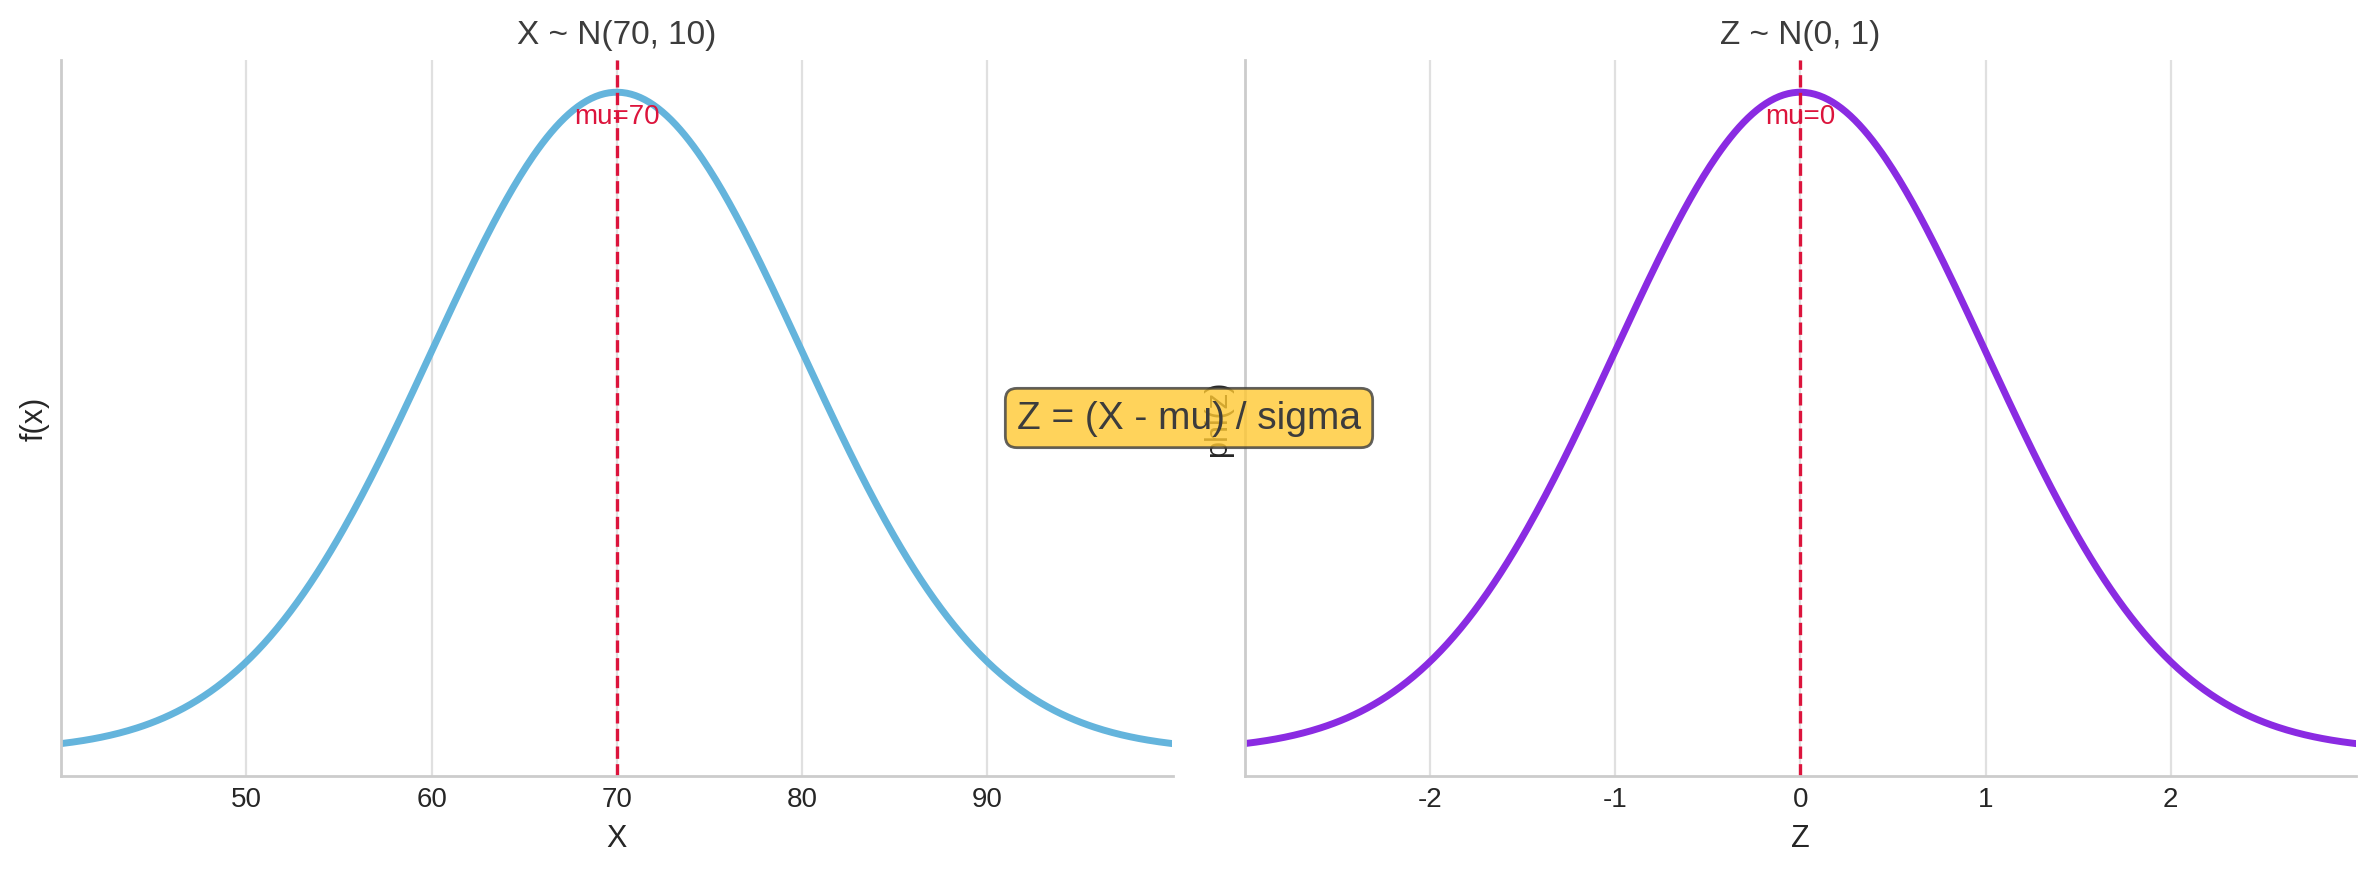
\includegraphics[width=0.95\linewidth]{fig_estandarizacion.png}
\end{center}
\end{frame}

% ============================================
% USO DE TABLAS Z - PARTE 1
% ============================================
\begin{frame}{Uso de Tablas de Distribución Normal (I)}
\begin{block}{Tabla Z (Lind, p. 782)}
La tabla proporciona el \textbf{área bajo la curva} desde $-\infty$ hasta un valor $Z$ dado:
$$P(Z \leq z) = \text{Área acumulada a la izquierda de } z$$
\end{block}

\begin{center}
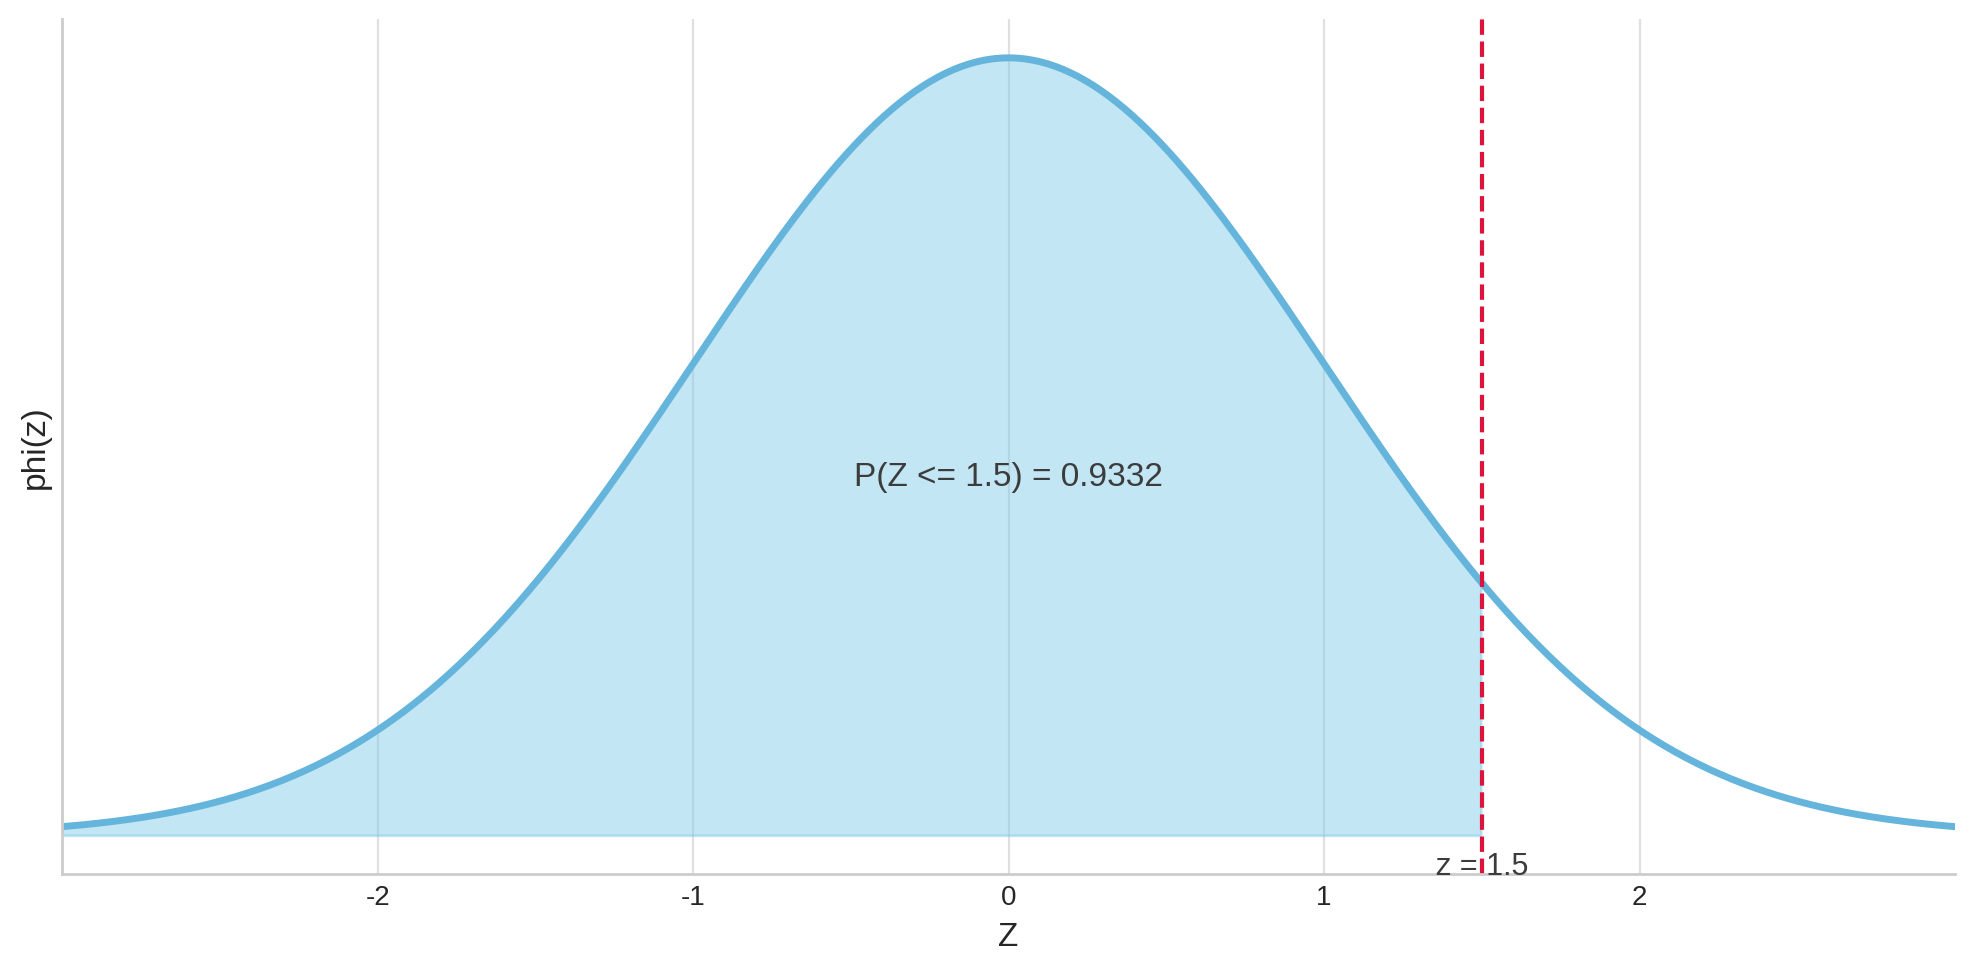
\includegraphics[width=0.80\linewidth]{fig_tabla_z.png}
\end{center}
\end{frame}

% ============================================
% USO DE TABLAS Z - PARTE 2
% ============================================
\begin{frame}{Uso de Tablas de Distribución Normal (II)}
\begin{alertblock}{Estructura de la tabla (Lind, p. 782)}
\begin{itemize}
  \item \textbf{Columna Z:} Valores de $Z$ (hasta 1 decimal)
  \item \textbf{Filas 0.00 a 0.09:} Segundo decimal de $Z$
  \item \textbf{Valor en celda:} Probabilidad acumulada $P(Z \leq z)$
\end{itemize}
\end{alertblock}

\vspace{0.2cm}
\begin{exampleblock}{Valores clave a memorizar}
\begin{center}
\begin{tabular}{c|c}
\toprule
\textbf{Z} & \textbf{Probabilidad acumulada} \\
\midrule
$1{,}645$ & $0{,}9500$ (90\% de confianza) \\
$1{,}96$ & $0{,}9750$ (95\% de confianza) \\
$2{,}576$ & $0{,}9950$ (99\% de confianza) \\
\bottomrule
\end{tabular}
\end{center}
\end{exampleblock}
\end{frame}

% ============================================
% EJEMPLO DE TABLA Z
% ============================================
\begin{frame}{Ejemplo: Lectura de Tabla Z}
\begin{exampleblock}{Ejemplo: Encontrar $P(Z \leq 1{,}96)$}
\textbf{Paso 1:} Buscar $Z = 1{,}9$ en la columna izquierda\\
\textbf{Paso 2:} Buscar $0{,}06$ en la fila superior\\
\textbf{Paso 3:} Intersección: $\boxed{P(Z \leq 1{,}96) = 0{,}9750}$
\end{exampleblock}

\begin{center}
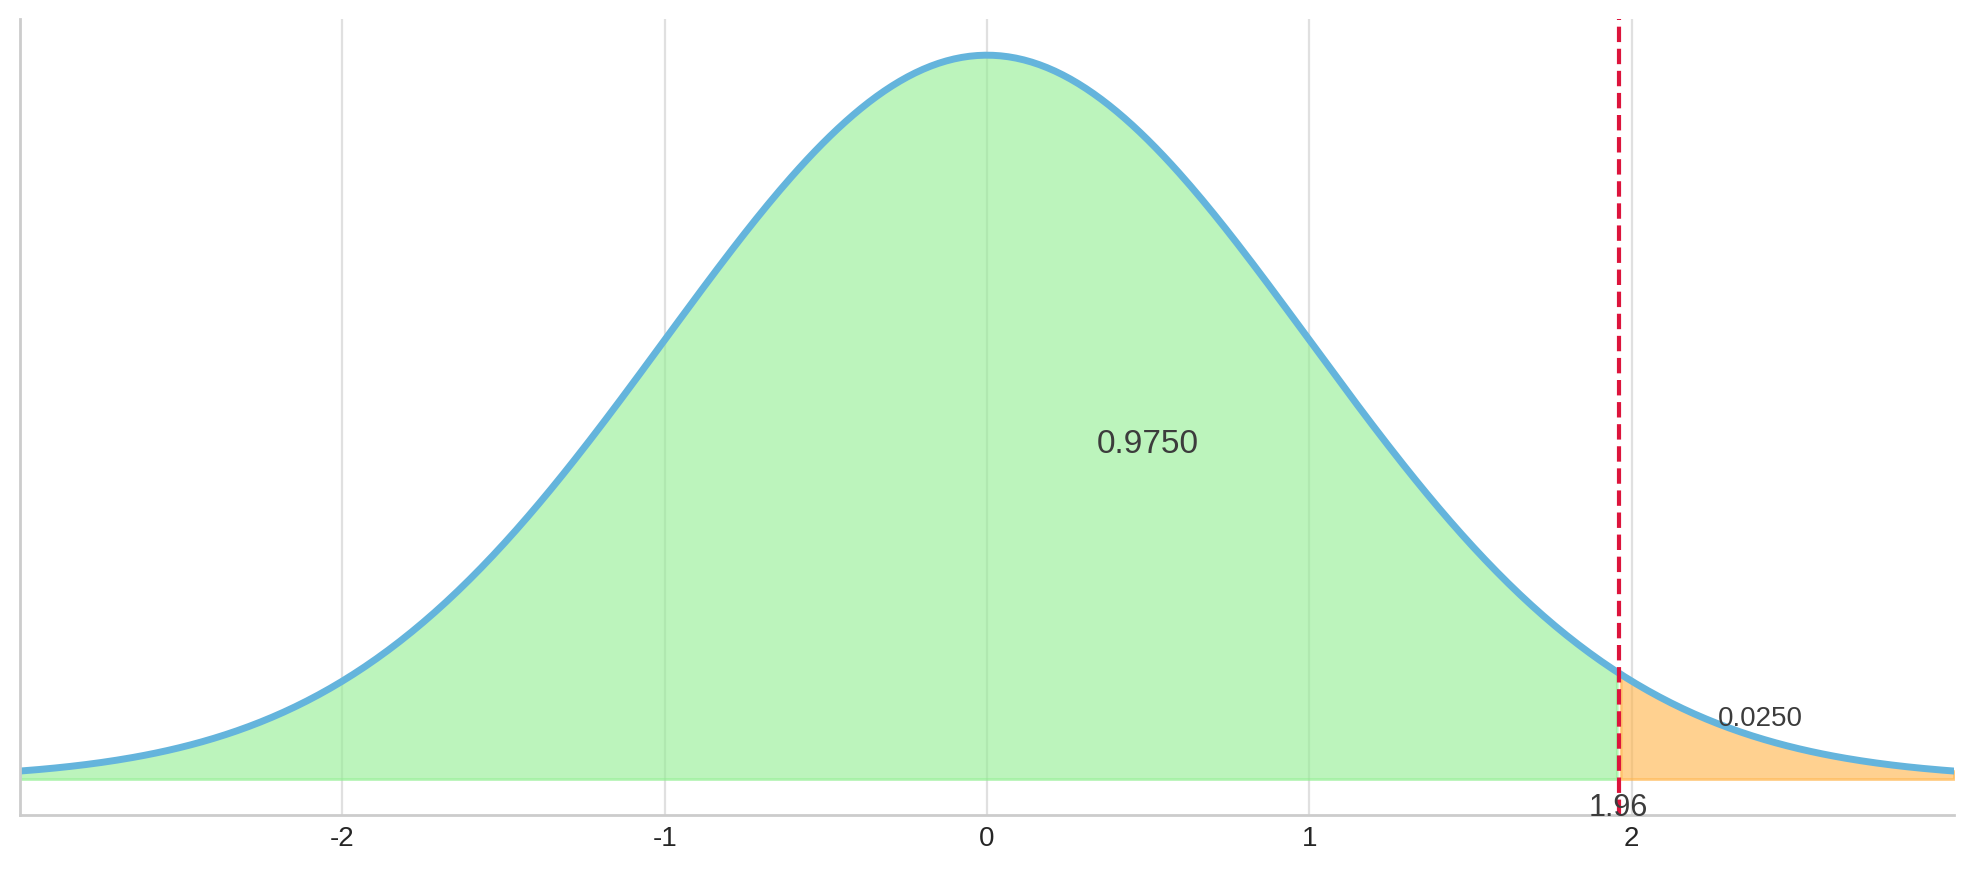
\includegraphics[width=0.80\linewidth]{fig_tabla_z_196.png}
\end{center}

\begin{block}{Interpretación}
El 97,5\% de los valores están por debajo de $Z = 1{,}96$, y el 2,5\% está por encima.
\end{block}
\end{frame}

% ============================================
% REGLA EMPÍRICA
% ============================================
\begin{frame}{Regla Empírica (68-95-99.7)}
\begin{block}{Para distribuciones normales:}
\begin{center}
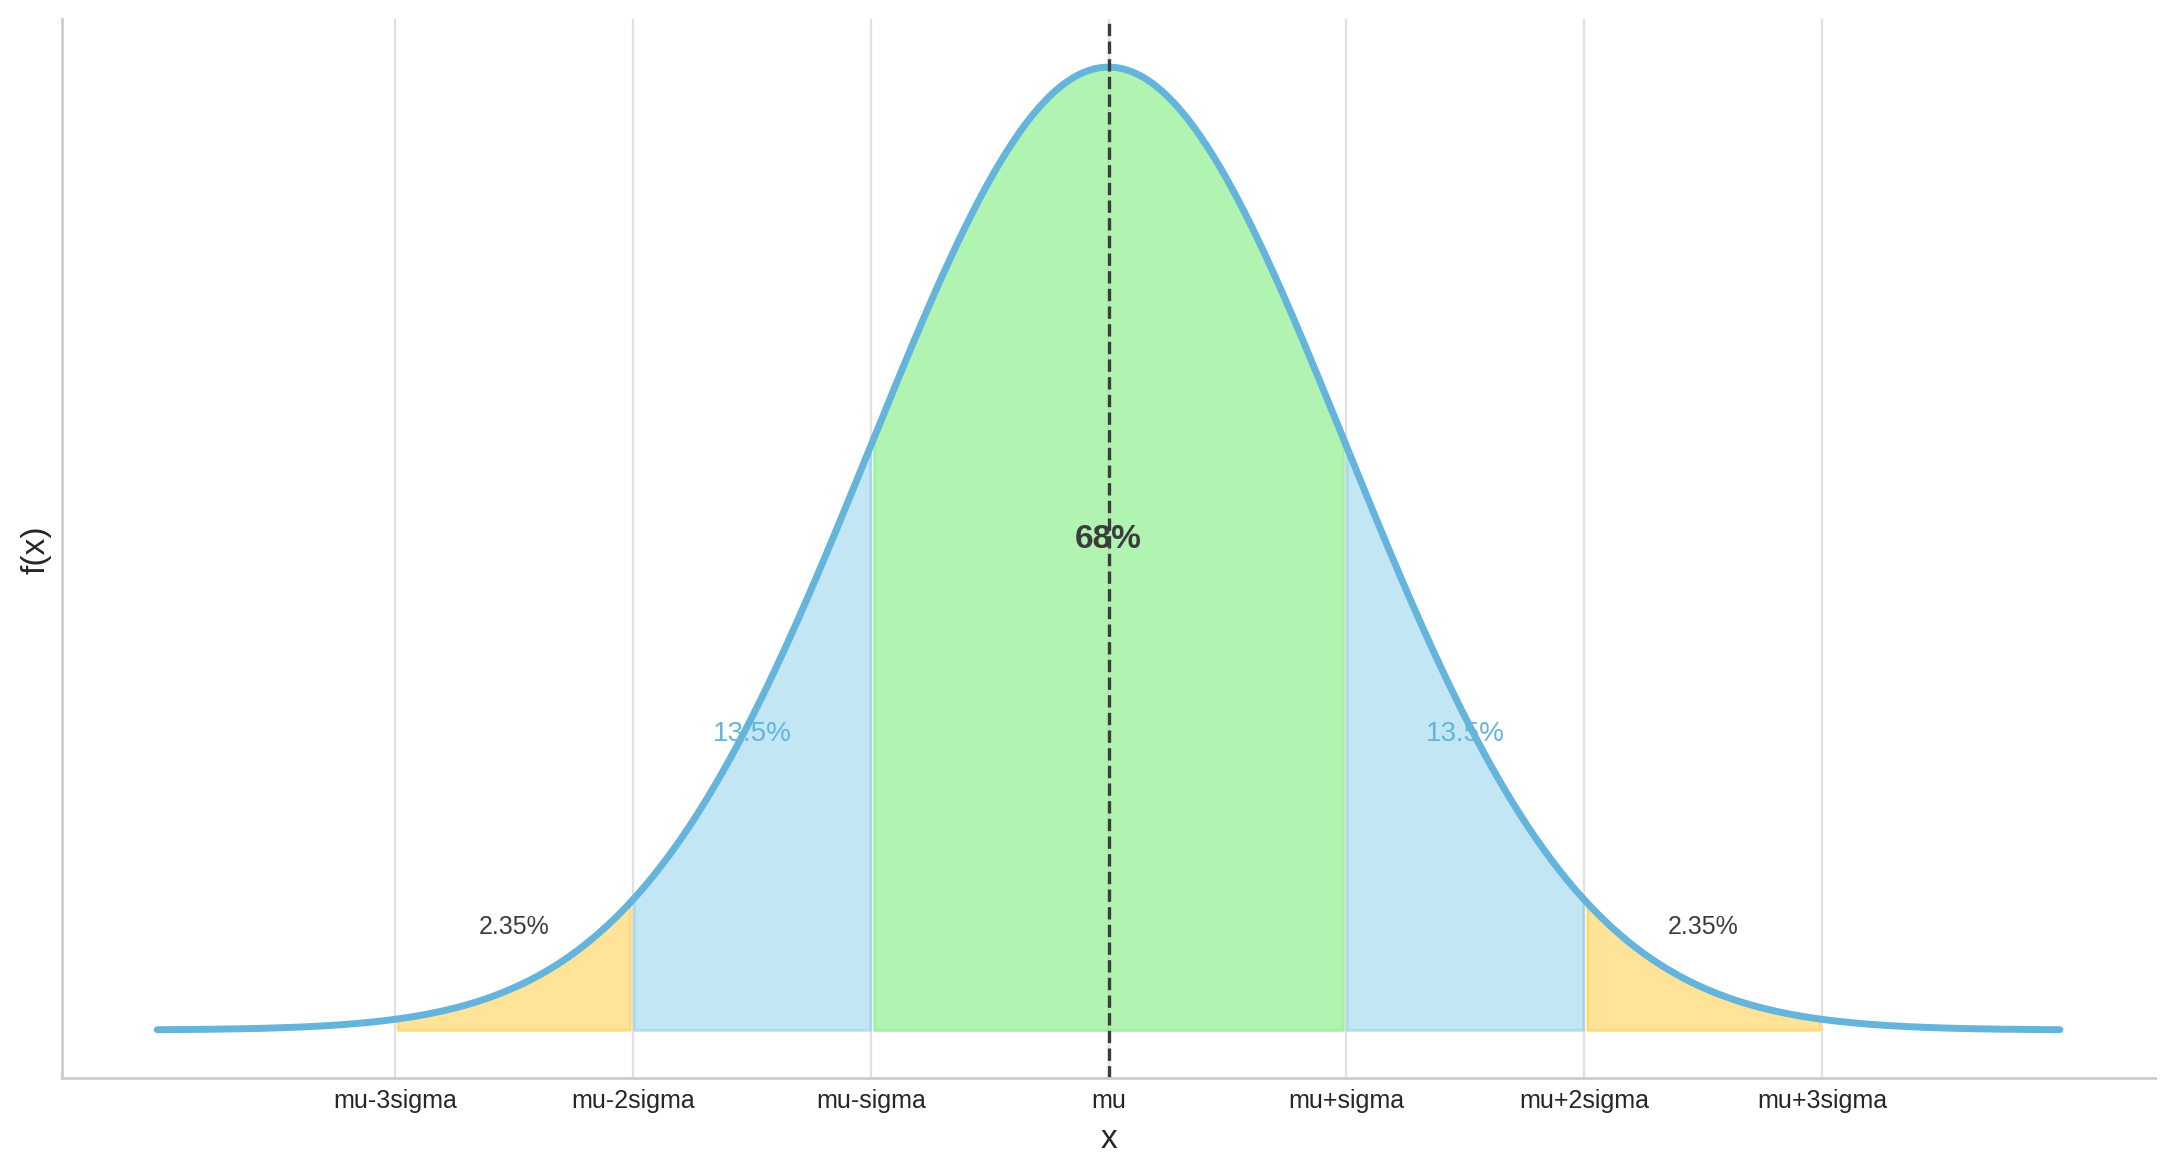
\includegraphics[width=0.95\linewidth]{fig_regla_empirica.png}
\end{center}
\end{block}

\begin{exampleblock}{Resumen}
\begin{itemize}
  \item $\mu \pm 1\sigma$: Aproximadamente \textbf{68\%} de los datos
  \item $\mu \pm 2\sigma$: Aproximadamente \textbf{95\%} de los datos
  \item $\mu \pm 3\sigma$: Aproximadamente \textbf{99,7\%} de los datos
\end{itemize}
\end{exampleblock}
\end{frame}

% ============================================
% EJERCICIO RESUELTO 1 - PARTE 1
% ============================================
\begin{frame}{Ejercicio Resuelto 1: Probabilidad Normal (I)}
\begin{exampleblock}{Problema (Lind, p. 233)}
El peso de los paquetes de café sigue una distribución normal con $\mu = 500$ g y $\sigma = 20$ g. ¿Cuál es la probabilidad de que un paquete pese menos de 530 g?
\end{exampleblock}

\vspace{0.2cm}
\begin{block}{\textbf{Paso 1:} Identificar datos}
\begin{itemize}
  \item $X = 530$ g (valor de interés)
  \item $\mu = 500$ g (media)
  \item $\sigma = 20$ g (desviación estándar)
\end{itemize}
\end{block}

\begin{block}{\textbf{Paso 2:} Estandarizar}
$$Z = \frac{X - \mu}{\sigma} = \frac{530 - 500}{20} = \frac{30}{20} = 1{,}5$$
\end{block}
\end{frame}

% ============================================
% EJERCICIO RESUELTO 1 - PARTE 2
% ============================================
\begin{frame}{Ejercicio Resuelto 1: Probabilidad Normal (II)}
\begin{block}{\textbf{Paso 3:} Buscar en tabla Z (Lind, p. 782)}
$$P(Z \leq 1{,}50) = 0{,}9332$$
\end{block}

\begin{exampleblock}{\textbf{Respuesta:}}
$$\boxed{P(X \leq 530) = 0{,}9332 \text{ o } 93{,}32\%}$$
\end{exampleblock}

\begin{center}
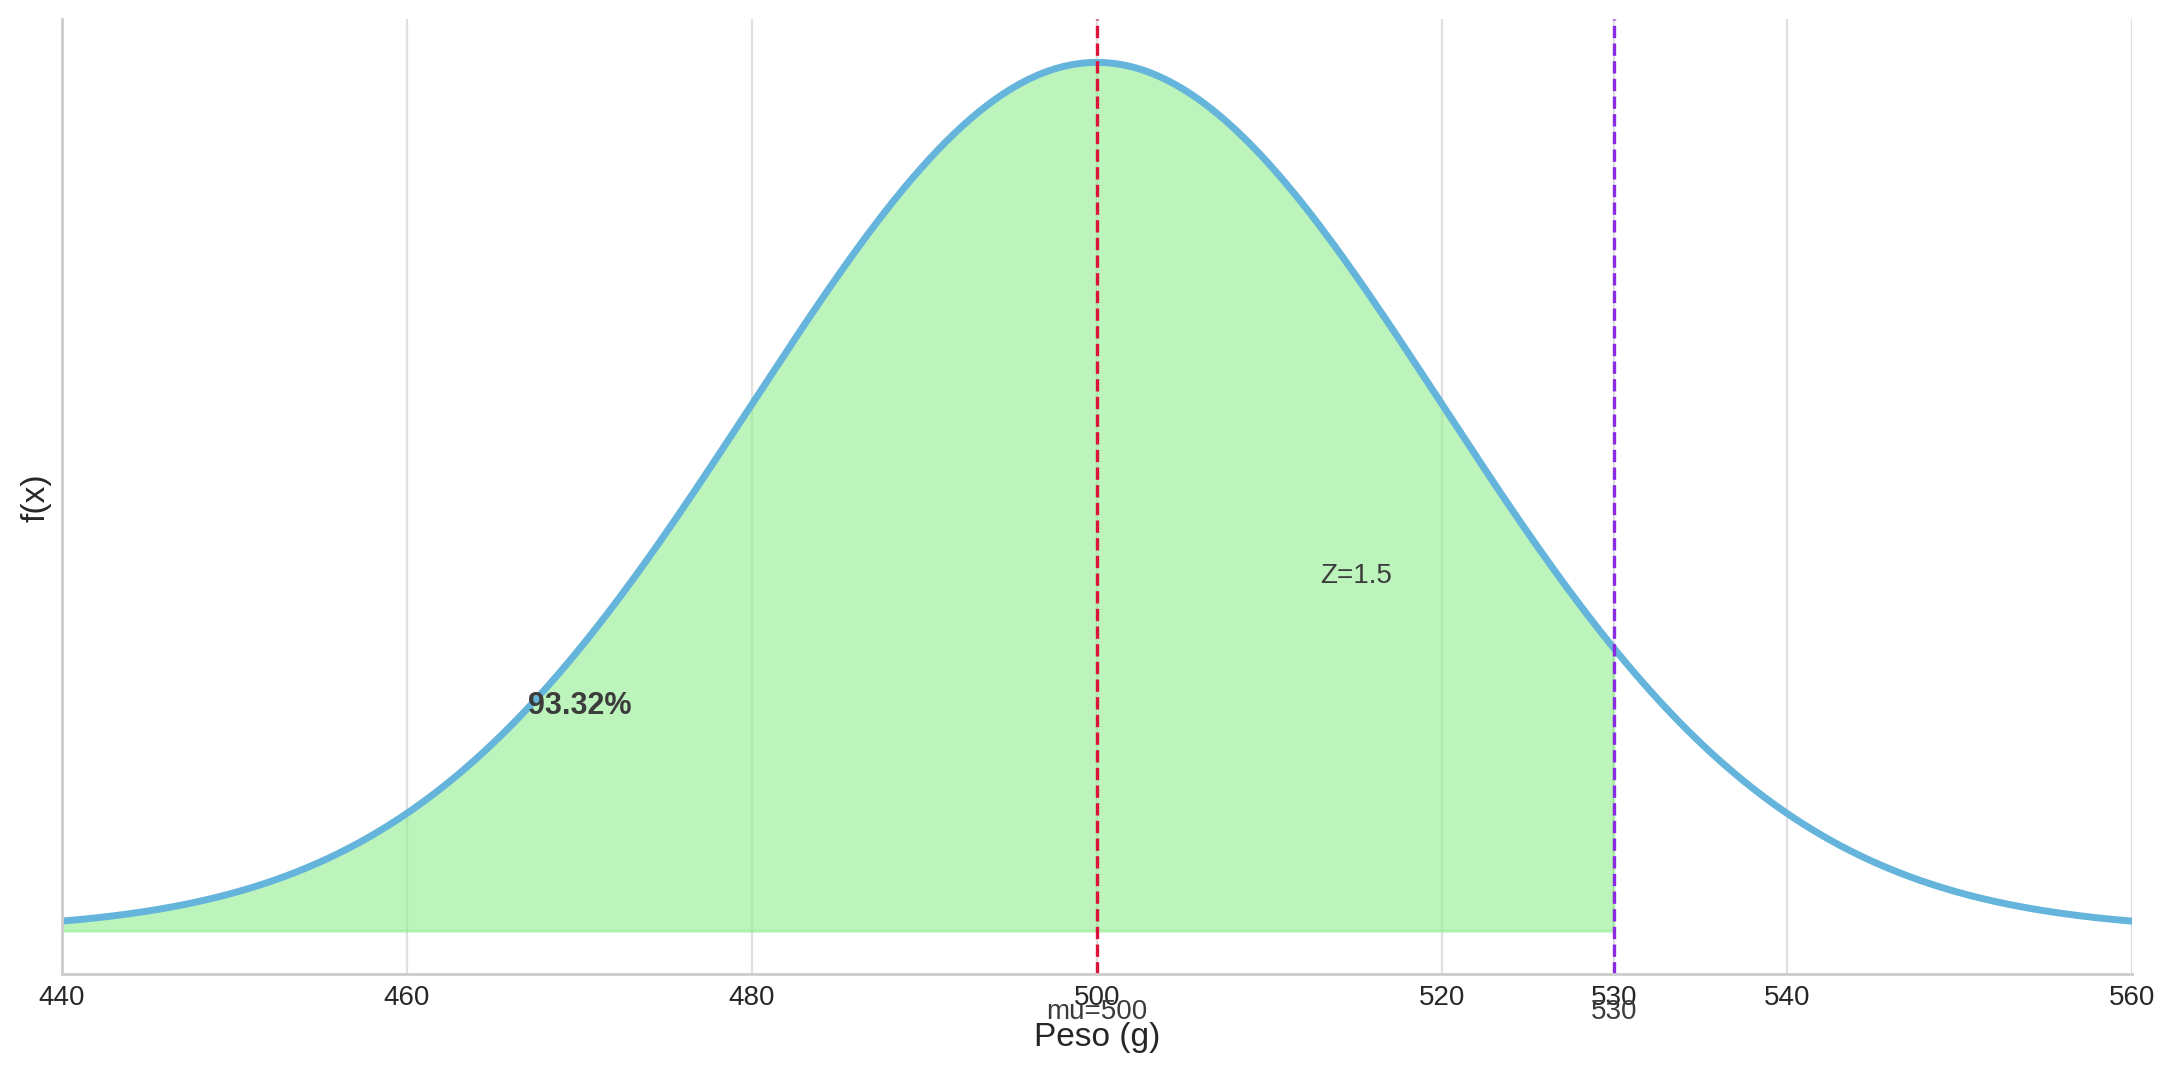
\includegraphics[width=0.85\linewidth]{fig_ejercicio1.png}
\end{center}

\begin{alertblock}{Interpretación}
Aproximadamente el \textbf{93,32\%} de los paquetes de café pesan menos de 530 g.
\end{alertblock}
\end{frame}

% ============================================
% EJERCICIO RESUELTO 2 - PARTE 1
% ============================================
\begin{frame}{Ejercicio Resuelto 2: Probabilidad entre dos valores (I)}
\begin{exampleblock}{Problema}
Los salarios iniciales de contadores públicos siguen $N(3500, 400)$ en Bs. ¿Qué porcentaje gana entre 3100 y 3900 Bs?
\end{exampleblock}

\vspace{0.2cm}
\begin{block}{\textbf{Paso 1:} Estandarizar ambos valores}
$$Z_1 = \frac{3100 - 3500}{400} = \frac{-400}{400} = -1{,}0$$
$$Z_2 = \frac{3900 - 3500}{400} = \frac{400}{400} = 1{,}0$$
\end{block}

\begin{block}{\textbf{Paso 2:} Buscar en tabla Z}
$$P(Z \leq 1{,}00) = 0{,}8413 \qquad P(Z \leq -1{,}00) = 0{,}1587$$
\end{block}
\end{frame}

% ============================================
% EJERCICIO RESUELTO 2 - PARTE 2
% ============================================
\begin{frame}{Ejercicio Resuelto 2: Probabilidad entre dos valores (II)}
\begin{block}{\textbf{Paso 3:} Calcular probabilidad del intervalo}
$$P(3100 \leq X \leq 3900) = P(-1 \leq Z \leq 1) = 0{,}8413 - 0{,}1587 = 0{,}6826$$
\end{block}

\begin{exampleblock}{\textbf{Respuesta:}}
$$\boxed{P(3100 \leq X \leq 3900) = 0{,}6826 \text{ o } 68{,}26\%}$$
\end{exampleblock}

\begin{center}
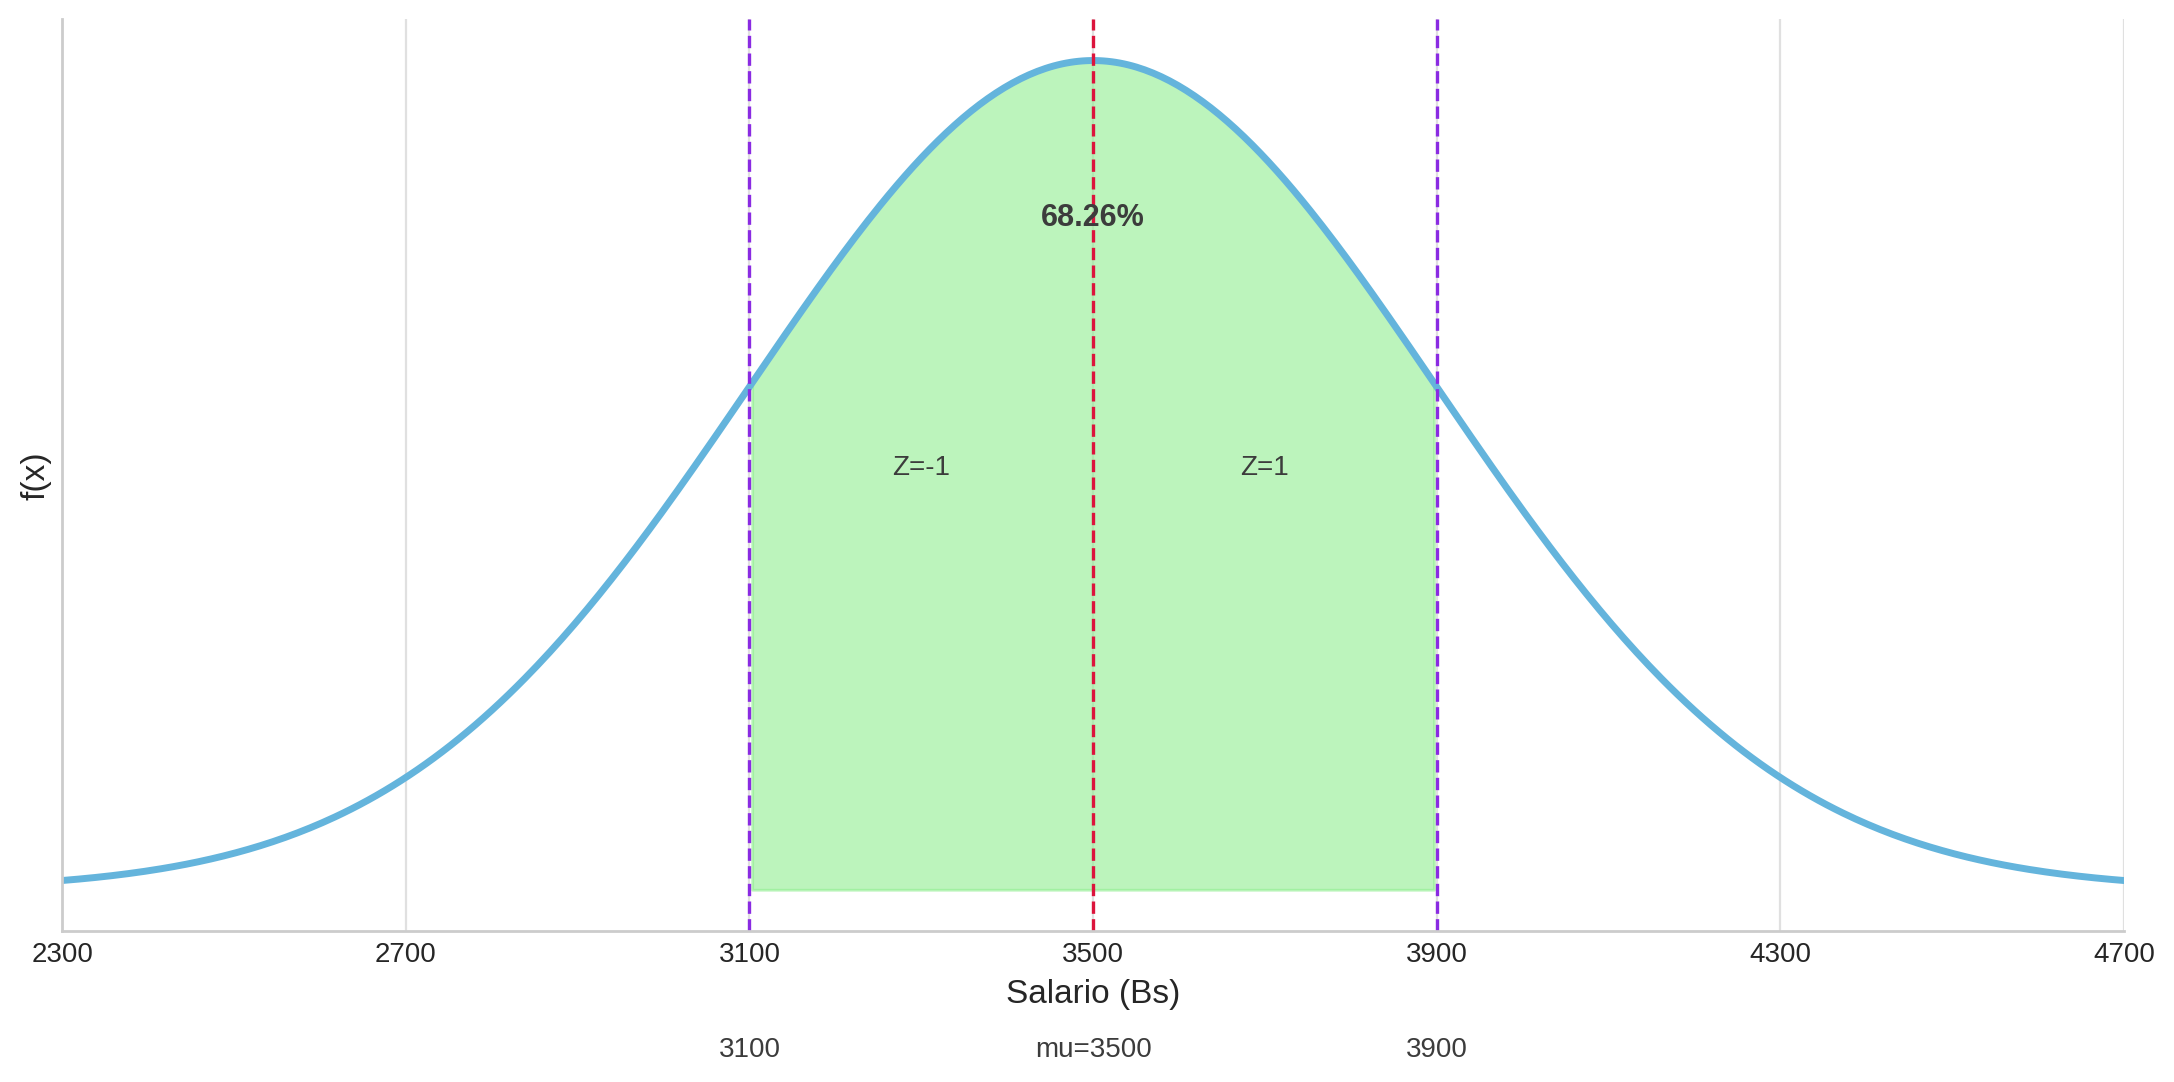
\includegraphics[width=0.85\linewidth]{fig_ejercicio2.png}
\end{center}

\begin{alertblock}{Observación}
Este resultado coincide con la \textbf{Regla Empírica}: $\mu \pm 1\sigma$ contiene aproximadamente 68\% de los datos.
\end{alertblock}
\end{frame}

% ============================================
% EJERCICIO RESUELTO 3 - PARTE 1
% ============================================
\begin{frame}{Ejercicio Resuelto 3: Cola derecha (I)}
\begin{exampleblock}{Problema}
El tiempo de servicio en un banco sigue $N(8, 2)$ minutos. ¿Cuál es la probabilidad de que el tiempo exceda 11 minutos?
\end{exampleblock}

\vspace{0.2cm}
\begin{block}{\textbf{Paso 1:} Estandarizar}
$$Z = \frac{11 - 8}{2} = \frac{3}{2} = 1{,}5$$
\end{block}

\begin{block}{\textbf{Paso 2:} Buscar en tabla Z}
$$P(Z \leq 1{,}50) = 0{,}9332$$
\end{block}

\begin{block}{\textbf{Paso 3:} Calcular cola derecha}
$$P(X > 11) = P(Z > 1{,}5) = 1 - P(Z \leq 1{,}5) = 1 - 0{,}9332 = 0{,}0668$$
\end{block}
\end{frame}

% ============================================
% EJERCICIO RESUELTO 3 - PARTE 2
% ============================================
\begin{frame}{Ejercicio Resuelto 3: Cola derecha (II)}
\begin{exampleblock}{\textbf{Respuesta:}}
$$\boxed{P(X > 11) = 0{,}0668 \text{ o } 6{,}68\%}$$
\end{exampleblock}

\begin{center}
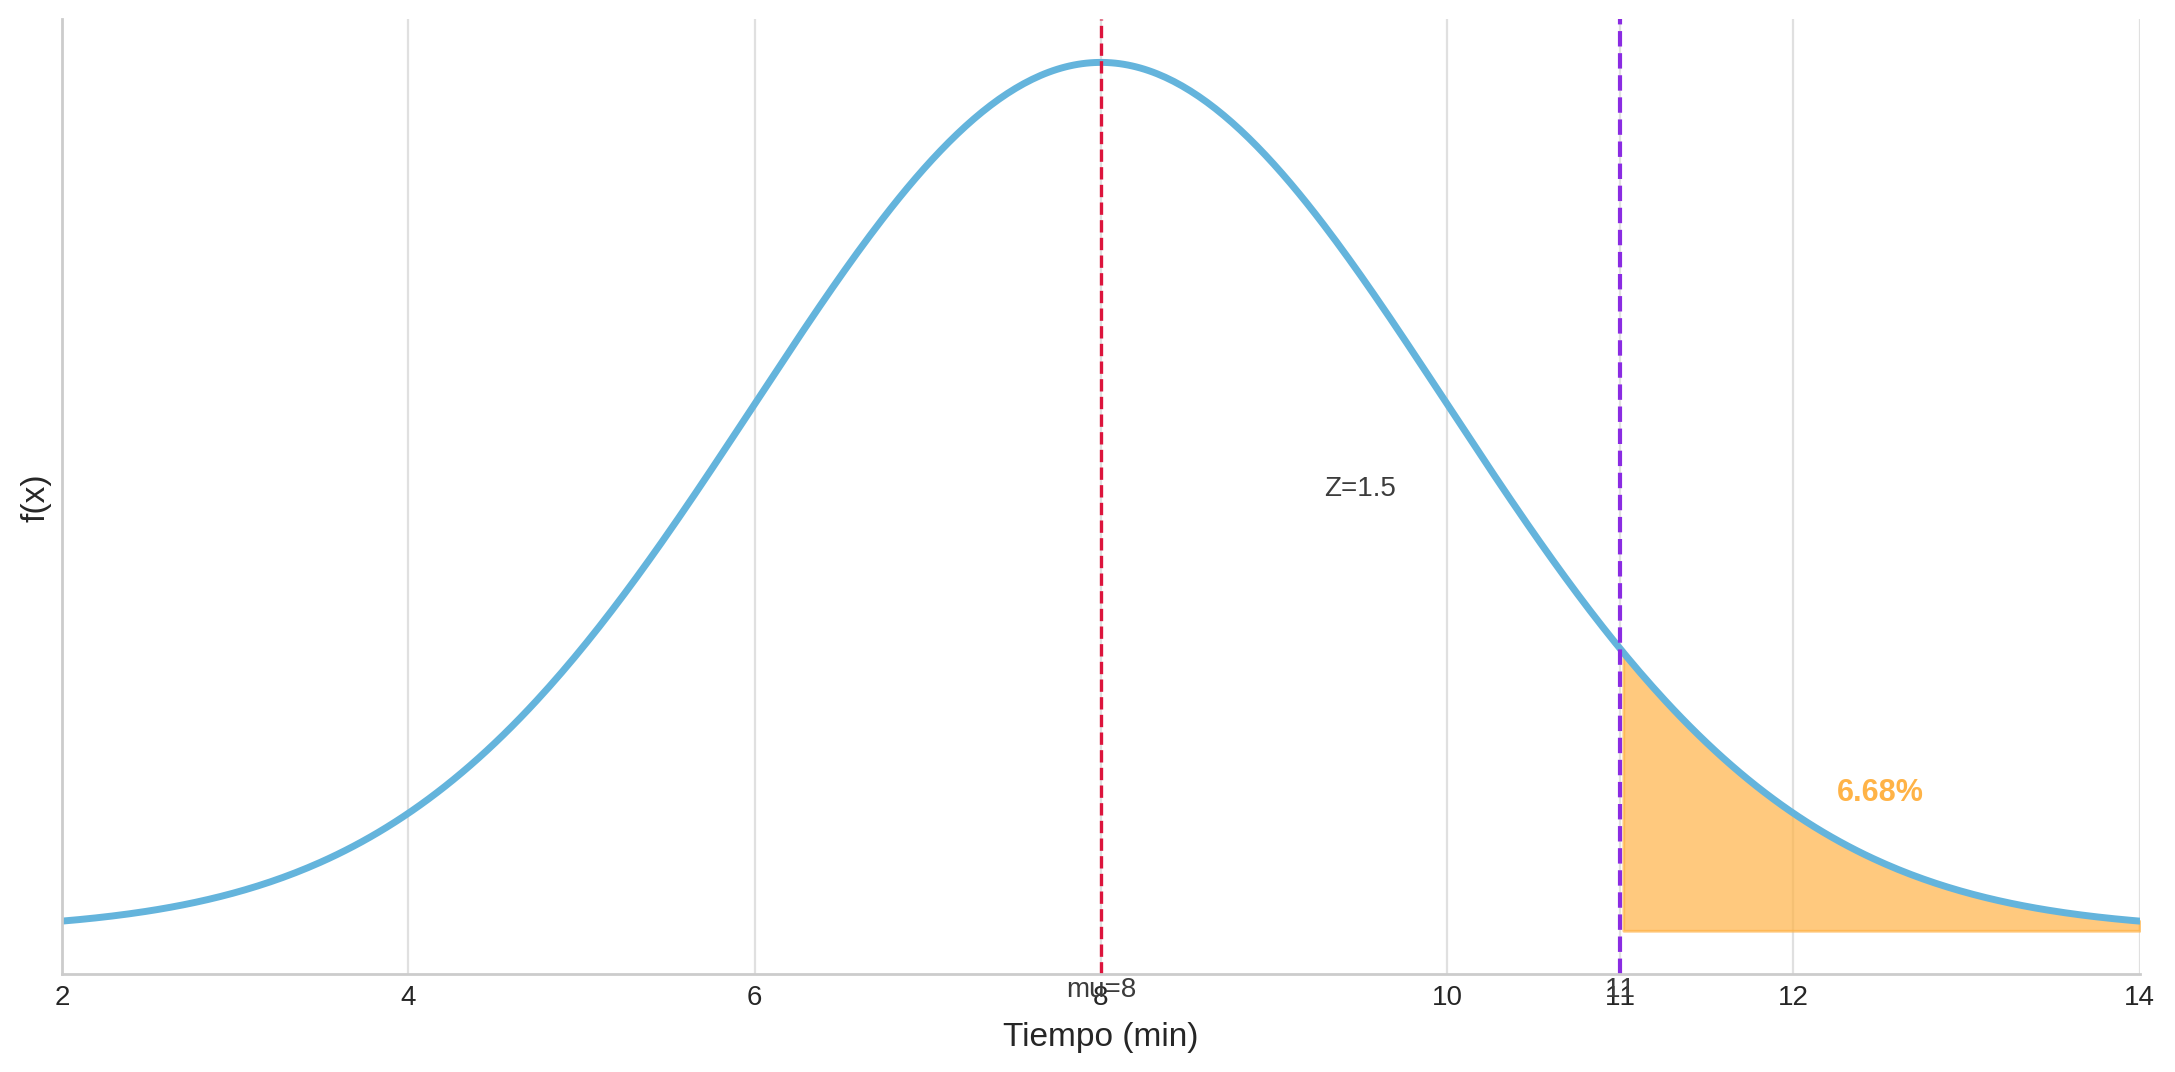
\includegraphics[width=0.85\linewidth]{fig_ejercicio3.png}
\end{center}

\vspace{0.2cm}
\begin{alertblock}{Fórmula general para cola derecha}
$$P(X > x) = 1 - P(Z \leq z) = 1 - \text{(valor de tabla)}$$
\end{alertblock}
\end{frame}

% ============================================
% RESUMEN DE FÓRMULAS
% ============================================
\begin{frame}{Resumen de Fórmulas Clave: Normal}
\begin{block}{Fórmulas Fundamentales}
\begin{center}
\begin{tabular}{>{\columncolor{celesteClaro}}l >{\columncolor{celesteClaro}}l}
\toprule
\textbf{Concepto} & \textbf{Fórmula} \\
\midrule
Función de densidad normal & $f(x) = \dfrac{1}{\sigma\sqrt{2\pi}} \cdot e^{-\frac{1}{2}\left(\frac{x-\mu}{\sigma}\right)^2}$ \\[0.4cm]
Estandarización & $Z = \dfrac{X - \mu}{\sigma}$ \\[0.4cm]
Probabilidad acumulada & $P(X \leq x) = P(Z \leq z)$ \\[0.3cm]
Probabilidad intervalo & $P(a \leq X \leq b) = P(Z_a \leq Z \leq Z_b)$ \\[0.3cm]
Cola derecha & $P(X > x) = 1 - P(Z \leq z)$ \\[0.3cm]
Cola izquierda & $P(X < x) = P(Z \leq z)$ \\
\bottomrule
\end{tabular}
\end{center}
\end{block}
\end{frame}

% ============================================
% TABLA Z RESUMEN
% ============================================
\begin{frame}{Tabla Z: Extracto (Lind, p. 782)}
\begin{block}{Cómo usar la tabla}
\begin{enumerate}
  \item Calcular $Z$ con la fórmula de estandarización
  \item Buscar fila con primer decimal de $Z$
  \item Buscar columna con segundo decimal
  \item Leer probabilidad acumulada
\end{enumerate}
\end{block}

\vspace{0.2cm}
\begin{center}
\footnotesize
\begin{tabular}{c|cccccc}
\toprule
\rowcolor{celeste}
$Z$ & 0{,}00 & 0{,}01 & 0{,}02 & 0{,}03 & 0{,}04 & 0{,}05 \\
\midrule
0{,}0 & 0{,}5000 & 0{,}5040 & 0{,}5080 & 0{,}5120 & 0{,}5160 & 0{,}5199 \\
0{,}5 & 0{,}6915 & 0{,}6950 & 0{,}6985 & 0{,}7019 & 0{,}7054 & 0{,}7088 \\
\rowcolor{verdePastel!30}
\textbf{1{,}0} & \textbf{0{,}8413} & 0{,}8438 & 0{,}8461 & 0{,}8485 & 0{,}8508 & 0{,}8531 \\
\rowcolor{verdePastel!30}
\textbf{1{,}5} & \textbf{0{,}9332} & 0{,}9345 & 0{,}9357 & 0{,}9370 & 0{,}9382 & 0{,}9394 \\
\rowcolor{verdePastel!30}
\textbf{2{,}0} & \textbf{0{,}9772} & 0{,}9778 & 0{,}9783 & 0{,}9788 & 0{,}9793 & 0{,}9798 \\
\rowcolor{verdePastel!30}
\textbf{2{,}5} & \textbf{0{,}9938} & 0{,}9940 & 0{,}9941 & 0{,}9943 & 0{,}9945 & 0{,}9946 \\
\bottomrule
\end{tabular}
\end{center}

\vspace{0.2cm}
\begin{exampleblock}{Valores clave a memorizar}
$Z = 1{,}645 \Rightarrow 90\%$ \quad $Z = 1{,}96 \Rightarrow 95\%$ \quad $Z = 2{,}576 \Rightarrow 99\%$
\end{exampleblock}
\end{frame}

% ============================================
% DISTRIBUCIÓN EXPONENCIAL - PARTE 1
% ============================================
\begin{frame}{Distribución Exponencial (I)}
\begin{block}{Definición}
Modela el \textbf{tiempo entre eventos} en un proceso de Poisson. Es continua, asimétrica y siempre positiva.
\end{block}

\vspace{0.2cm}
\begin{exampleblock}{Función de Densidad}
$$f(x) = \lambda e^{-\lambda x} \quad \text{para } x > 0$$
Donde $\lambda$ es la tasa promedio de ocurrencia por unidad de tiempo.
\end{exampleblock}

\vspace{0.2cm}
\begin{block}{Propiedades}
\begin{itemize}
  \item Media: $\mu = \dfrac{1}{\lambda}$
  \item Desviación estándar: $\sigma = \dfrac{1}{\lambda}$
  \item No necesita tablas: se usa la función exponencial directamente
\end{itemize}
\end{block}
\end{frame}

% ============================================
% DISTRIBUCIÓN EXPONENCIAL - PARTE 2
% ============================================
\begin{frame}{Distribución Exponencial (II)}
\begin{center}
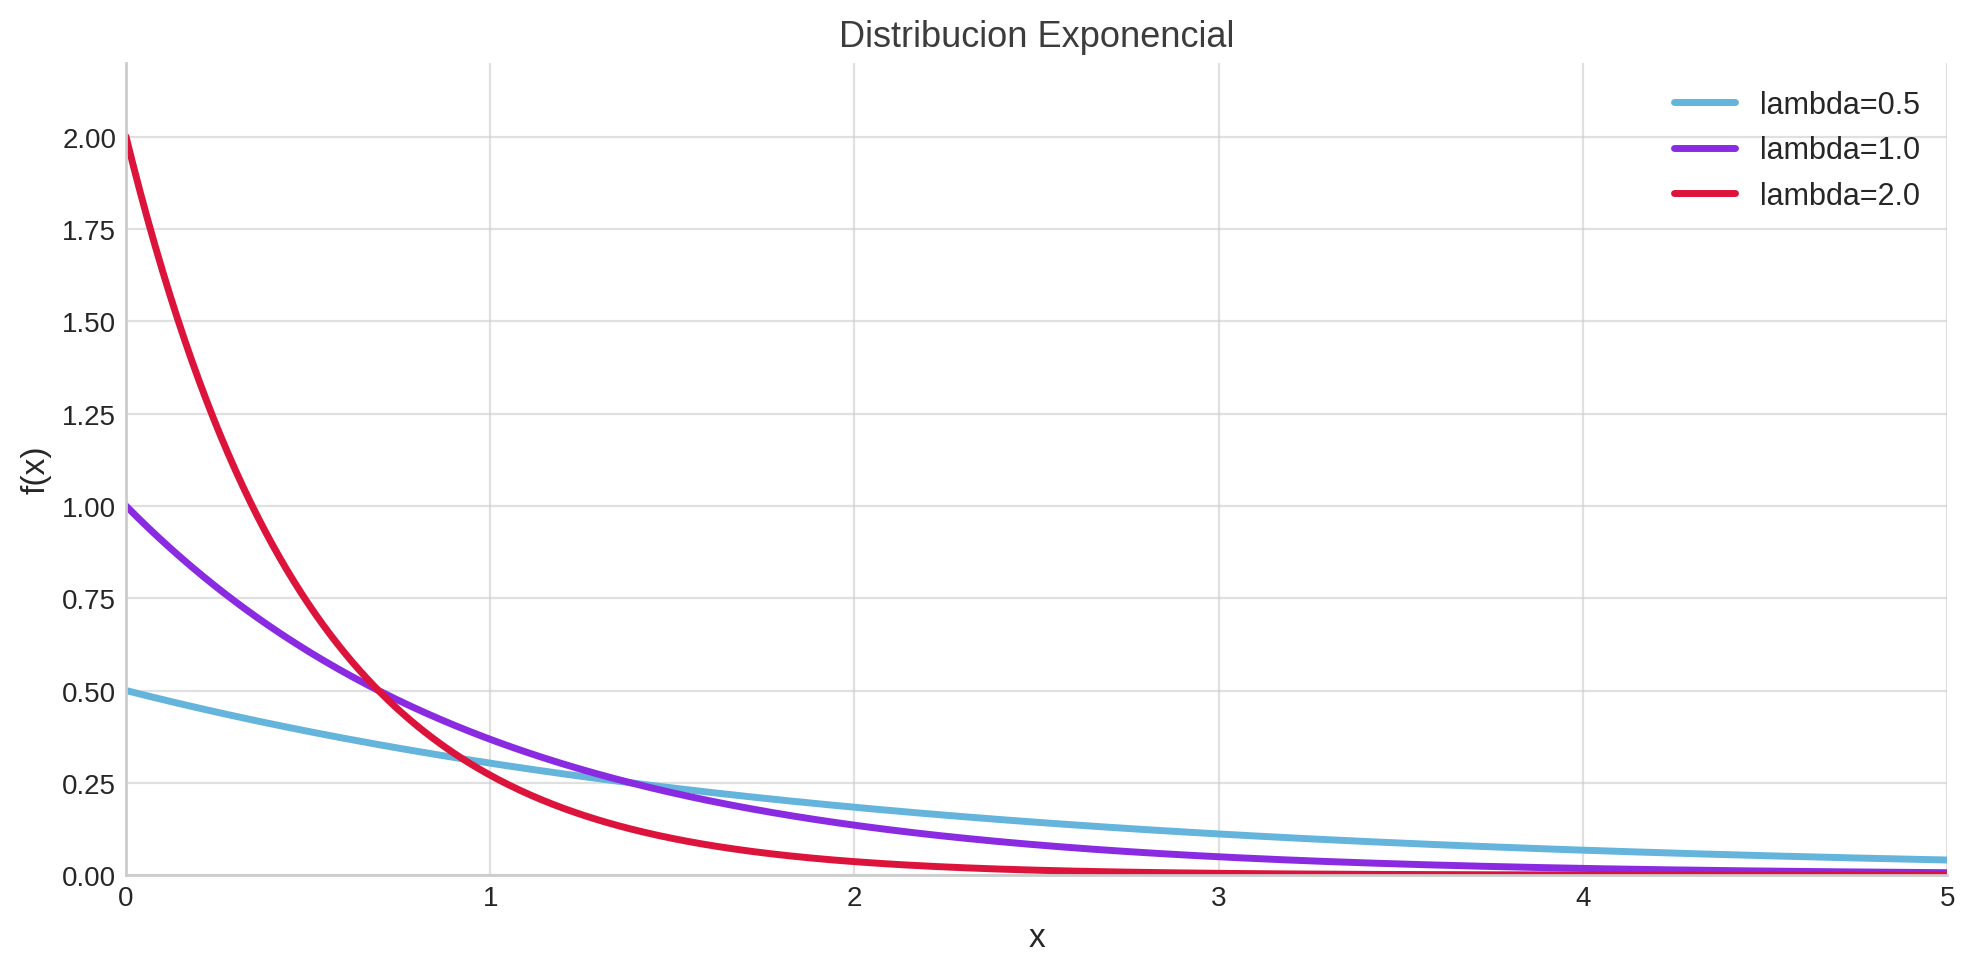
\includegraphics[width=0.85\linewidth]{fig_exponencial.png}
\end{center}

\vspace{0.2cm}
\begin{alertblock}{Fórmulas clave (sin tabla necesaria)}
$$P(X > x) = e^{-\lambda x} \qquad P(X \leq x) = 1 - e^{-\lambda x}$$
\end{alertblock}
\end{frame}

% ============================================
% CASOS REALES EXPONENCIAL
% ============================================
\begin{frame}{Casos Reales: Distribución Exponencial}
\begin{columns}[T]
\begin{column}{0.48\textwidth}
\begin{block}{Aplicaciones típicas}
\begin{enumerate}
  \item \textbf{Tiempo entre fallas} de una máquina
  \item \textbf{Tiempo de servicio} en atención al cliente
  \item Vida útil de componentes electrónicos
  \item Tiempo entre llegadas a un servidor
\end{enumerate}
\end{block}
\end{column}
\begin{column}{0.48\textwidth}
\begin{exampleblock}{Caso real: Call Center}
\footnotesize
Un call center recibe llamadas a razón de $\lambda = 4$ llamadas/hora.

\textbf{Pregunta:} ¿Probabilidad de esperar más de 30 minutos entre llamadas?

$$P(X > 0{,}5) = e^{-4 \times 0{,}5} = e^{-2} = 0{,}1353$$

\textbf{Respuesta:} 13{,}53\% de probabilidad
\end{exampleblock}
\end{column}
\end{columns}
\end{frame}

% ============================================
% EJERCICIO EXPONENCIAL
% ============================================
\begin{frame}{Ejercicio: Distribución Exponencial}
\begin{exampleblock}{Problema}
La vida útil de un fusible sigue una distribución exponencial con media de 1000 horas. ¿Cuál es la probabilidad de que dure más de 1200 horas?
\end{exampleblock}

\vspace{0.2cm}
\begin{block}{\textbf{Paso 1:} Identificar parámetros}
Media = 1000 h $\Rightarrow$ $\lambda = \frac{1}{1000} = 0{,}001$
\end{block}

\begin{block}{\textbf{Paso 2:} Aplicar fórmula}
$$P(X > 1200) = e^{-\lambda x} = e^{-0{,}001 \times 1200} = e^{-1{,}2}$$
\end{block}

\begin{block}{\textbf{Paso 3:} Calcular}
$$e^{-1{,}2} = 0{,}3012$$
\end{block}

\begin{exampleblock}{\textbf{Respuesta:}}
$$\boxed{P(X > 1200) = 0{,}3012 \approx 30{,}12\%}$$
\end{exampleblock}
\end{frame}

% ============================================
% COMPARATIVO DE DISTRIBUCIONES
% ============================================
\begin{frame}{Comparativo: Normal vs Exponencial}
\begin{center}
\footnotesize
\begin{tabular}{>{\columncolor{celesteClaro}}p{3cm} >{\columncolor{verdePastel!20}}p{5cm} >{\columncolor{fucsiaPastel!20}}p{5cm}}
\toprule
\textbf{Característica} & \textbf{Normal} & \textbf{Exponencial} \\
\midrule
Variable & Continua & Continua (tiempo) \\
Parámetros & $\mu$, $\sigma$ & $\lambda$ \\
Forma & Simétrica, campana & Asimétrica, decaimiento \\
Uso principal & Prob. generales, aproximaciones & Tiempos de espera, vida útil \\
Tablas & Z (p. 782 Lind) & No necesita tablas \\
Ejemplo real & Alturas, calificaciones, salarios & Fallas de equipo, servicios \\
\bottomrule
\end{tabular}
\end{center}
\end{frame}

% ============================================
% CASOS REALES INTEGRADOS - NORMAL
% ============================================
\begin{frame}{Caso Real Integrado: Normal}
\begin{exampleblock}{Caso: Banco}
\footnotesize
El tiempo de atención al cliente sigue $N(8, 2)$ minutos. Si el banco tiene 200 clientes/día, ¿cuántos esperan más de 12 minutos?

$Z = (12-8)/2 = 2$ \quad $P(Z > 2) = 1 - 0{,}9772 = 0{,}0228$

\textbf{Respuesta:} $200 \times 0{,}0228 \approx 5$ clientes/día
\end{exampleblock}

\vspace{0.3cm}
\begin{exampleblock}{Caso: Calidad de producción}
\footnotesize
Una máquina empaqueta café con $\mu = 500$ g y $\sigma = 20$ g. De 1000 paquetes, ¿cuántos se espera que pesen entre 480 y 520 g?

$Z_1 = -1$, $Z_2 = 1$ \quad $P(-1 \leq Z \leq 1) = 0{,}6826$

\textbf{Respuesta:} $1000 \times 0{,}6826 \approx 683$ paquetes
\end{exampleblock}
\end{frame}

% ============================================
% CASOS REALES INTEGRADOS - EXPONENCIAL
% ============================================
\begin{frame}{Caso Real Integrado: Exponencial}
\begin{exampleblock}{Caso: Seguros}
\footnotesize
Una aseguradora sabe que reclamos ocurren cada 30 días en promedio ($\lambda = 1/30$). ¿Probabilidad de pasar 60 días sin reclamos?

$P(X > 60) = e^{-(1/30) \times 60} = e^{-2} = 0{,}1353$

\textbf{Respuesta:} 13{,}53\% de probabilidad
\end{exampleblock}

\vspace{0.3cm}
\begin{exampleblock}{Caso: Mantenimiento}
\footnotesize
Una máquina tiene vida útil media de 5000 horas. ¿Probabilidad de que falle antes de las 3000 horas?

$\lambda = 1/5000$ \quad $P(X \leq 3000) = 1 - e^{-0{,}0002 \times 3000} = 1 - e^{-0{,}6} = 0{,}4512$

\textbf{Respuesta:} 45{,}12\% de probabilidad de falla antes de 3000 h
\end{exampleblock}
\end{frame}

% ============================================
% RESUMEN FINAL
% ============================================
\begin{frame}{Resumen de la Unidad 4}
\begin{columns}[T]
\begin{column}{0.48\textwidth}
\begin{block}{Distribución Normal}
\begin{itemize}
  \item Campana de Gauss, simétrica
  \item Estandarización: $Z = \frac{X-\mu}{\sigma}$
  \item Tabla Z (Lind, p. 782)
  \item Regla empírica: 68-95-99.7
\end{itemize}
\end{block}
\end{column}
\begin{column}{0.48\textwidth}
\begin{exampleblock}{Distribución Exponencial}
\begin{itemize}
  \item Tiempos de espera, vida útil
  \item $P(X > x) = e^{-\lambda x}$
  \item No requiere tablas
  \item Media = Desv. std = $1/\lambda$
\end{itemize}
\end{exampleblock}
\end{column}
\end{columns}

\vspace{0.3cm}
\begin{alertblock}{Referencias bibliográficas}
\begin{itemize}
  \item \textbf{Texto del curso:} MSc. Anselmo Salguero Arano. Unidad 4.
  \item \textbf{Lind, Marchal, Wathen.} \textit{Estadística Aplicada}. 15 Ed. McGraw-Hill, 2012.
  \begin{itemize}
    \item Cap. 7: Distribuciones Continuas (pp. 222--264)
    \item Apéndice B: Tablas (p. 782)
  \end{itemize}
\end{itemize}
\end{alertblock}
\end{frame}

% ============================================
% CIERRE
% ============================================
\begin{frame}[plain]
\begin{center}
\vspace{2cm}
{\Huge\textcolor{celeste}{\textbf{¡Gracias!}}}

\vspace{1cm}
{\Large\textcolor{grisOscuro}{¿Preguntas?}}

\vspace{2cm}
\begin{tikzpicture}
\draw[celesteBorde, thick, rounded corners=10pt, fill=celesteClaro] (0,0) rectangle (8,2);
\node at (4,1) {\large\textcolor{grisOscuro}{MSc. Anselmo Salguero Arano}};
\end{tikzpicture}

\vspace{0.5cm}
{\footnotesize\textcolor{grisOscuro}{Estadística II -- MAT-260\\
Universidad Autónoma Gabriel René Moreno}}
\end{center}
\end{frame}

\end{document}
